\section{Auswertung}
\label{sec:Auswertung}

\subsection{Diffferentielle Energieverteilung der Elektronen}

\begin{figure}[H]
  \centering
  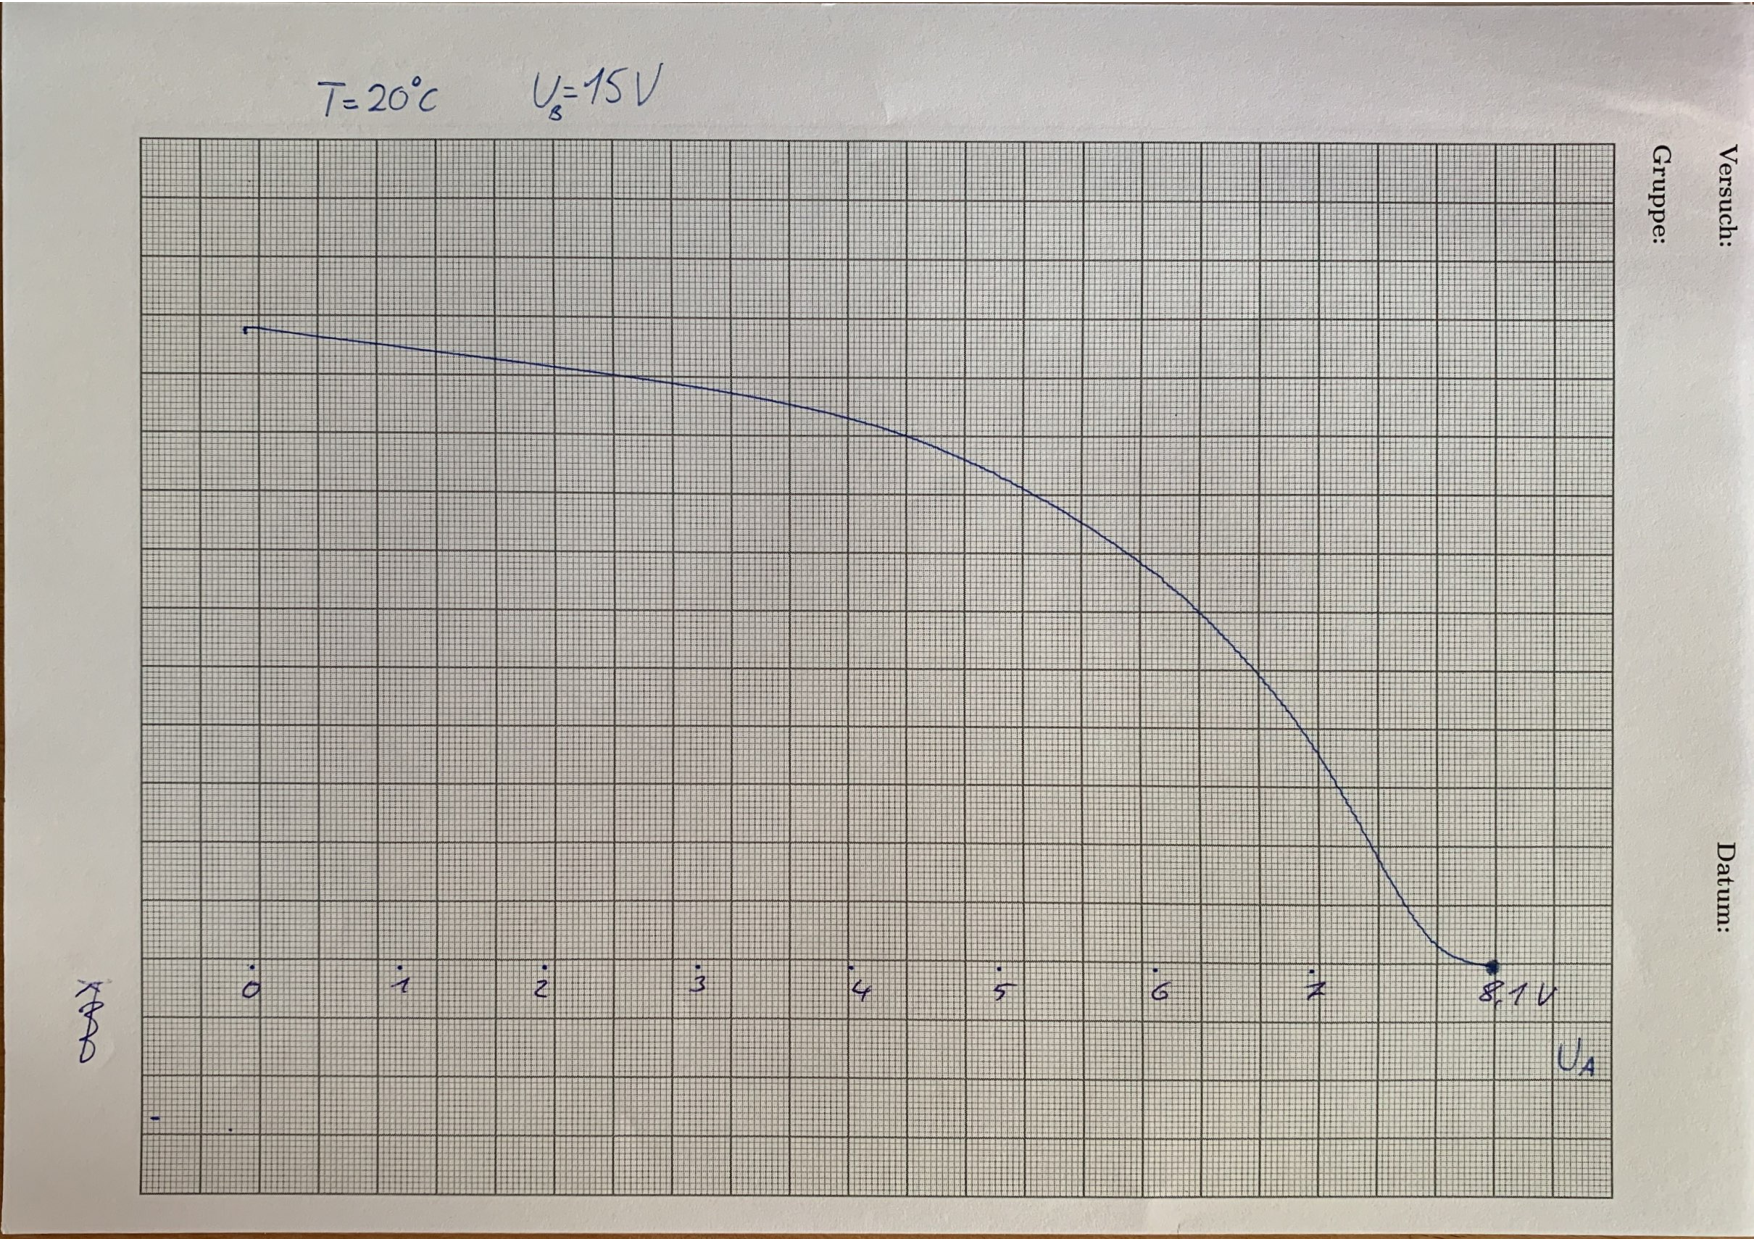
\includegraphics[height=8cm]{content/pics/originaldaten/1.pdf}
  \caption{Aufgezeichnete Integrale Energieverteilung der Elektronen $T=20\,\unit{\celsius}$.}
  \label{fig:Int Energie 20 Grad}
\end{figure}

\begin{table}[H]
  \centering
  \caption{Abgelesene Wertepaare für $U_A$ und $\symup{\Delta}I_A$ aus 10 Steigungsdreiecken in \autoref{fig:Int Energie 20 Grad}}
  \label{tab:Diff Energie 20 Grad}
  \begin{tabular}{S[table-format=1.1] S[table-format=1.1] S[table-format=2.0]}
      \toprule
       {$U_A\,/\,\unit{\volt}$} & {$\symup{\Delta}U_A\,/\,\unit{\volt}$} & {$\symup{\Delta}I_A\,/\,\unit{\ampere}$} \\
      \midrule
      0.0 & 0.5 &	3 \\
      0.5 & 0.5 &	2 \\
      1.0 & 0.5 &	2 \\
      1.5 & 0.5 &	1 \\
      2.0 & 0.5 &	2 \\
      2.5 & 0.5 &	2 \\
      3.0 & 0.5 &	2 \\
      3.5 & 0.5 &	3 \\
      4.0 & 0.5 &	4 \\
      4.5 & 0.5 &	6 \\
      5.0 & 0.5 &	7 \\
      5.5 & 0.5 &	9 \\
      6.0 & 0.5 &	12 \\
      6.5 & 0.5 &	18 \\
      7.0 & 0.5 &	23 \\
      7.5 & 0.5 &	14 \\
      \bottomrule 
  \end{tabular}
\end{table}

\begin{figure}[H]
    \centering
    \includegraphics[height=8cm]{build/Differentielle_Energie_20Grad.pdf}
    \caption{Differentielle Energieverteilng der Elektronen bei $T=20\,\unit{\celsius}$.}
    \label{fig:Diff Energie 20Grad}
\end{figure}

\begin{figure}[H]
  \centering
  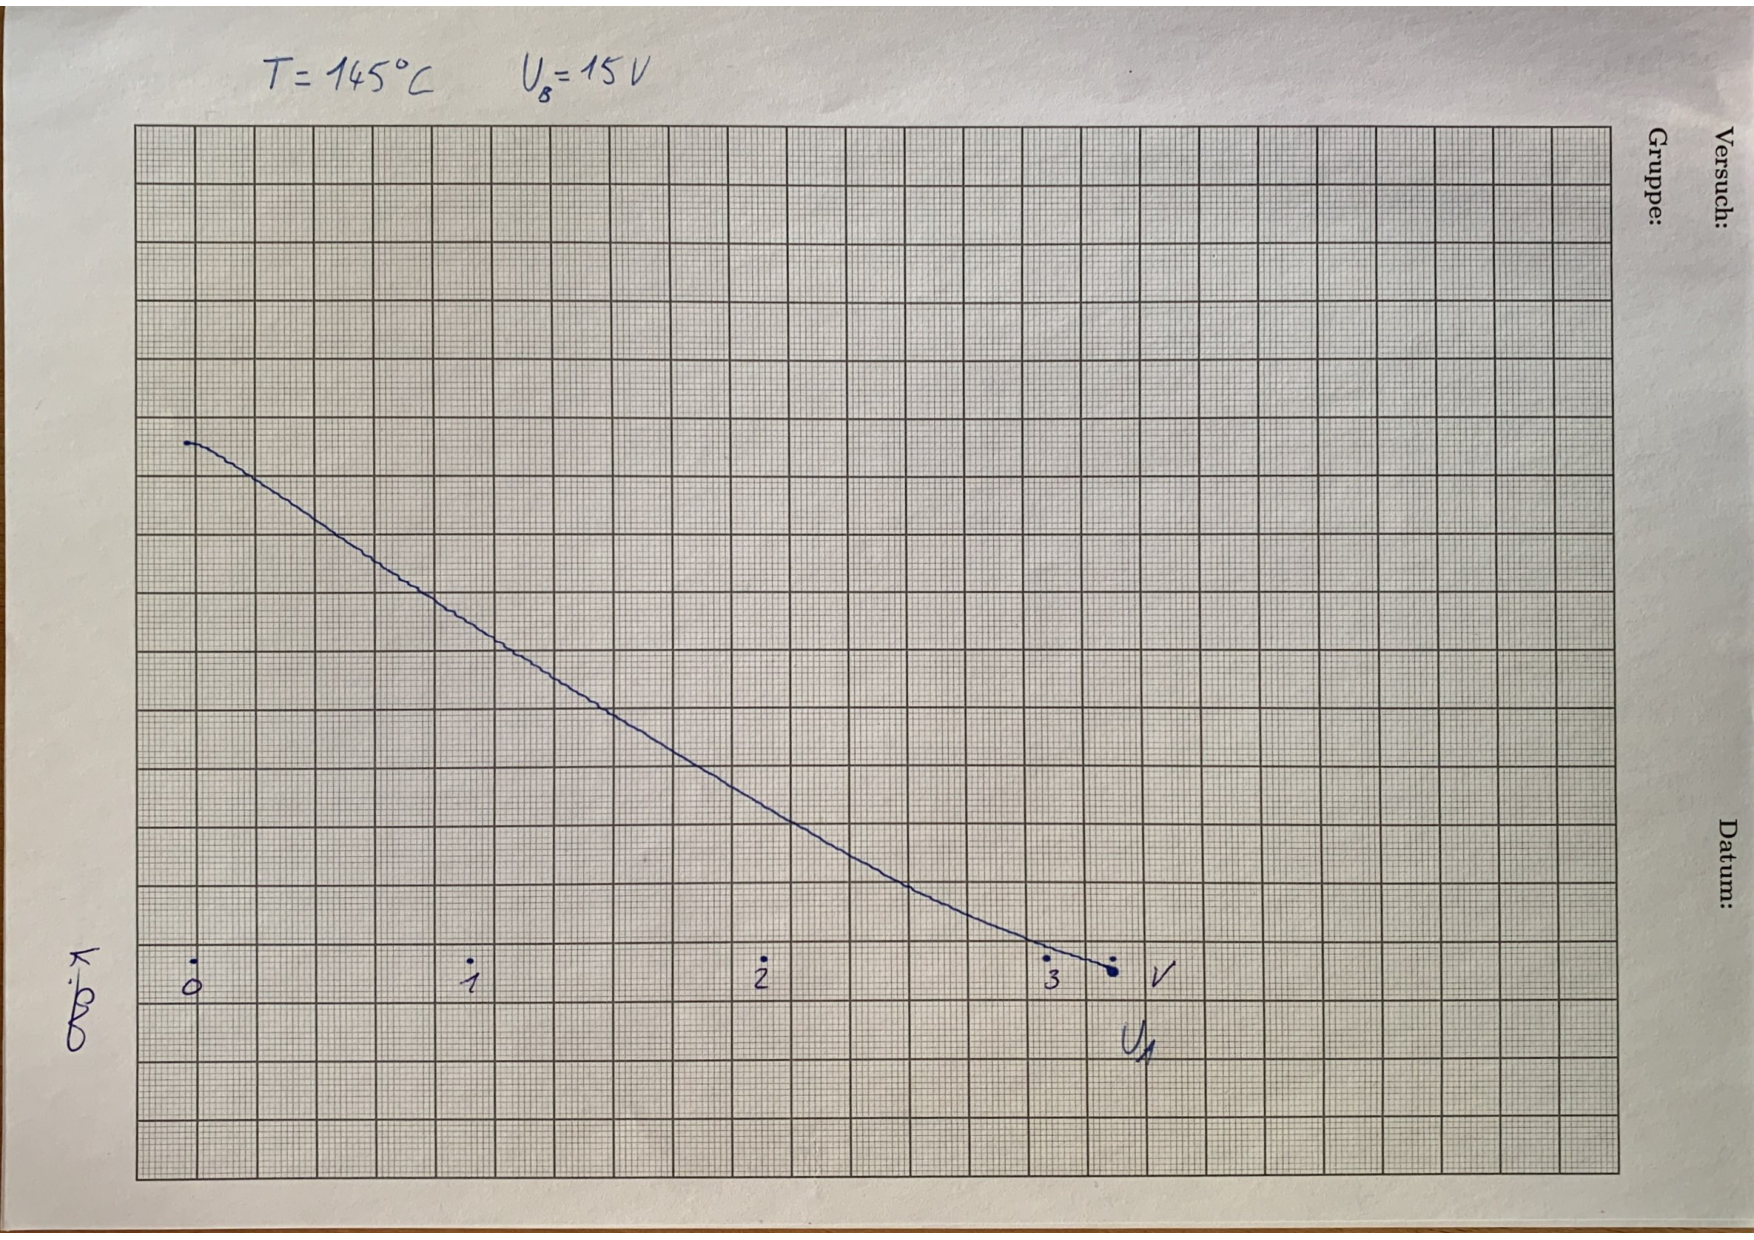
\includegraphics[height=8cm]{content/pics/originaldaten/2.pdf}
  \caption{Aufgezeichnete Integrale Energieverteilung der Elektronen $T=145\,\unit{\celsius}$.}
  \label{fig:Int Energie 145 Grad}
\end{figure}

\begin{table}[H]
  \centering
  \caption{Abgelesene Wertepaare für $U_A$ und $\symup{\Delta}I_A$ aus 4 Steigungsdreiecken in \autoref{fig:Int Energie 145 Grad}}
  \label{tab:Diff Energie 145 Grad}
  \begin{tabular}{S[table-format=1.1] S[table-format=1.1] S[table-format=2.0]}
      \toprule
       {$U_A\,/\,\unit{\volt}$} & {$\symup{\Delta}U_A\,/\,\unit{\volt}$} & {$\symup{\Delta}I_A\,/\,\unit{\ampere}$} \\
      \midrule
      0.0 & 0.5 &	15 \\
      0.5 & 0.5 &	15 \\
      1.0 & 0.5 &	16 \\
      1.5 & 0.5 &	17 \\
      2.0 & 0.5 &	14 \\
      \bottomrule 
  \end{tabular}
\end{table}


\begin{figure}[H]
    \centering
    \includegraphics[height=8cm]{build/Differentielle_Energie_145Grad.pdf}
    \caption{Differentielle Energieverteilng der Elektronen bei $T=145\,\unit{\celsius}$.}
    \label{fig:Diff Energie 145Grad}
\end{figure}



\subsection{Franck-Hertz Kurve}

\begin{figure}[H]
  \centering
  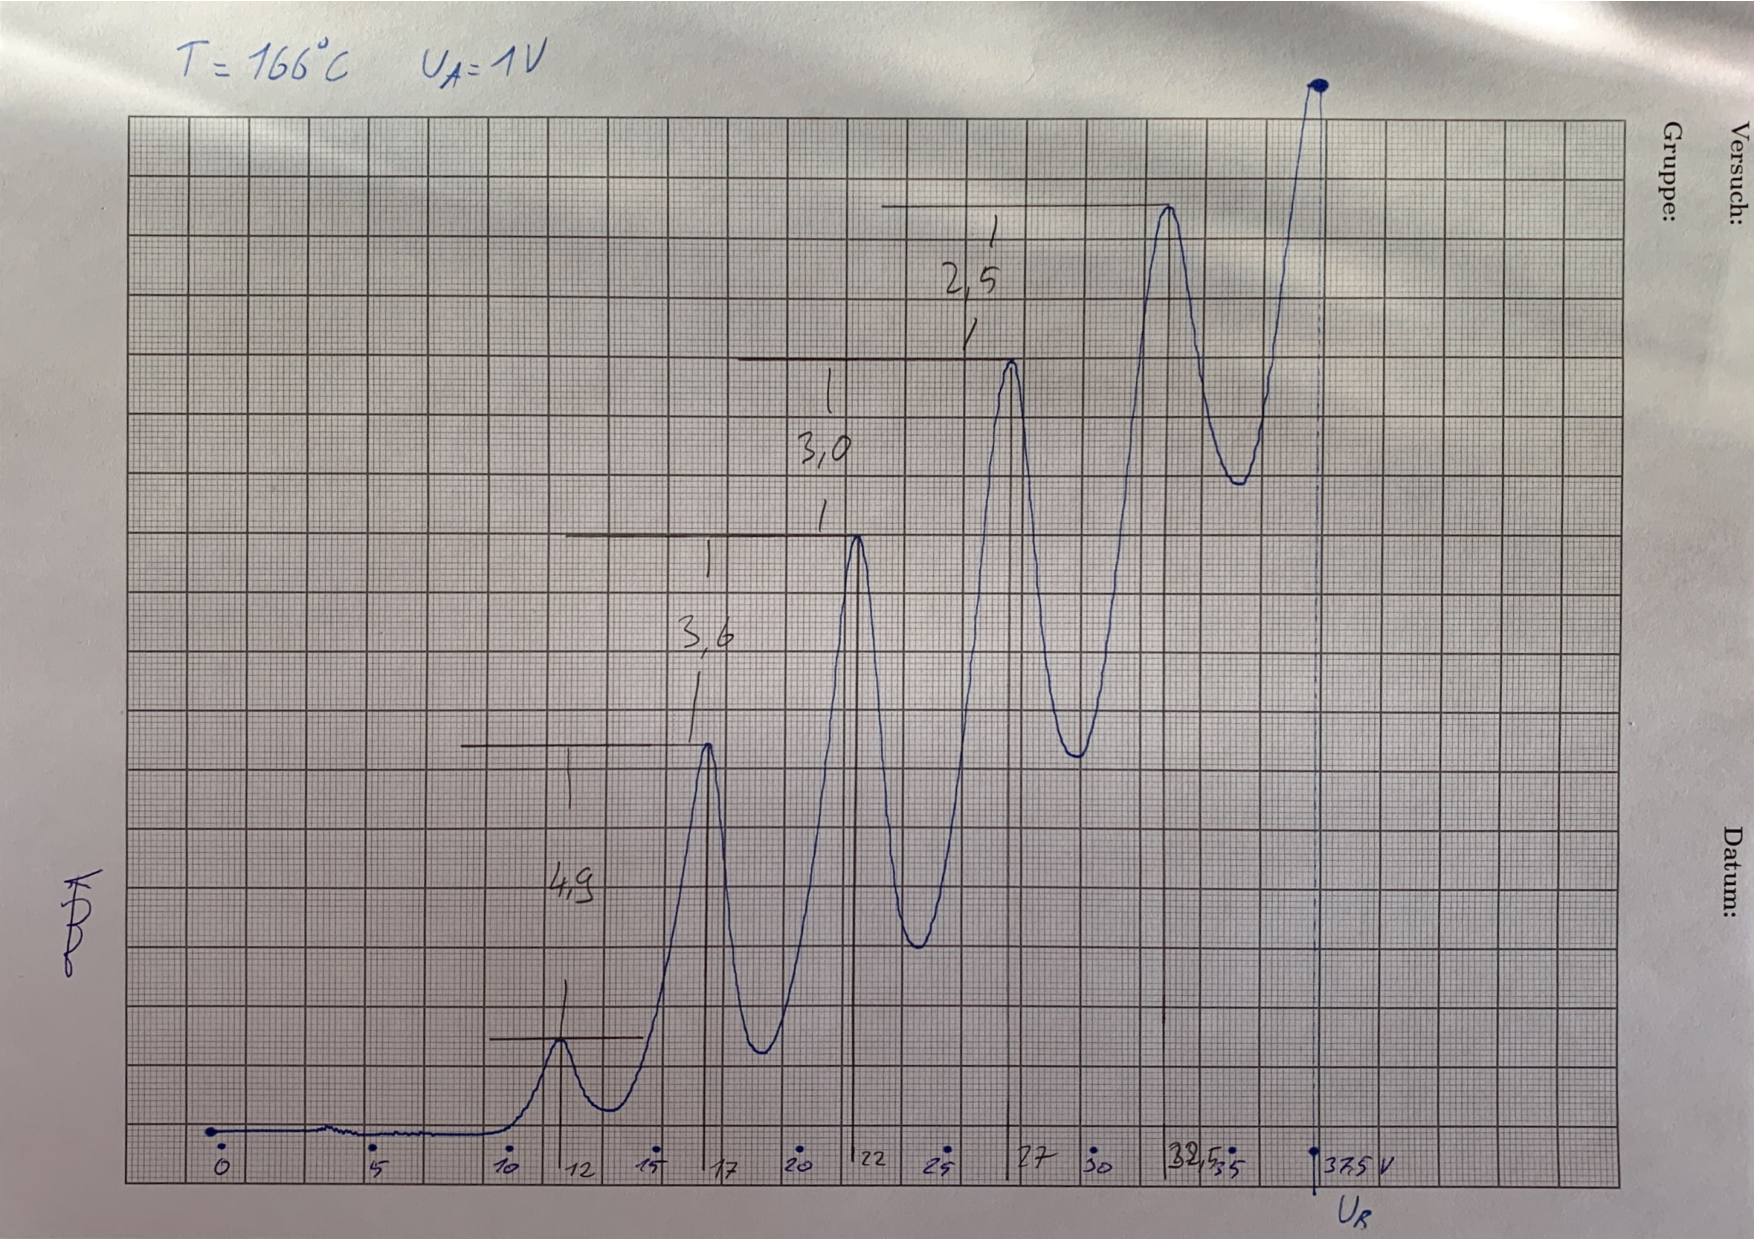
\includegraphics[height=8cm]{content/data/FH_166.pdf}
  \caption{Aufgezeichnete Franck-Hertz Kurve bei $T=166\,\unit{\celsius}$.}
  \label{fig:FHZ 166Grad}
\end{figure}

\begin{figure}[H]
  \centering
  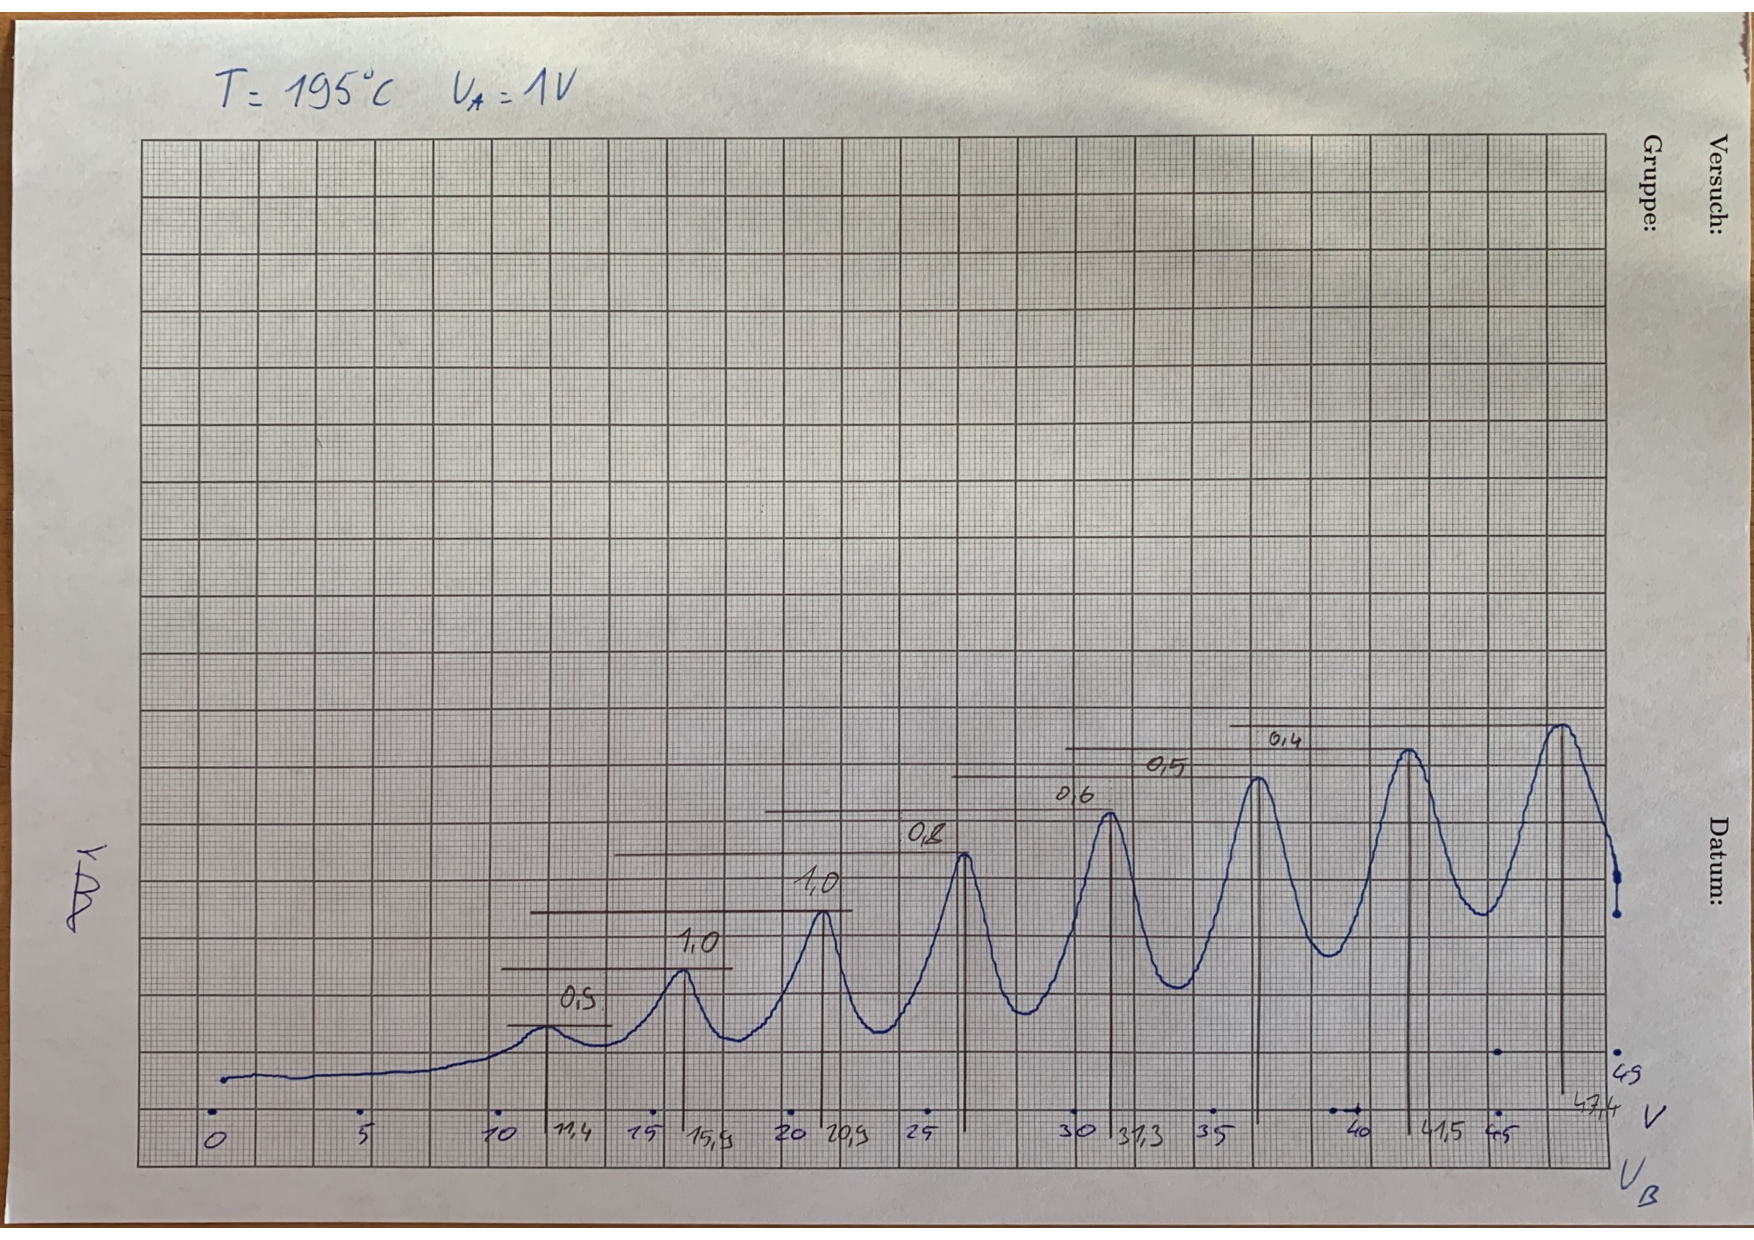
\includegraphics[height=8cm]{content/data/FH_195.pdf}
  \caption{Aufgezeichnete Franck-Hertz Kurve bei $T=195\,\unit{\celsius}$.}
  \label{fig:FHZ 195Grad}
\end{figure}